\documentclass{article}

\usepackage{fullpage}
\usepackage{graphicx}
\usepackage{amsfonts, amsmath}
\usepackage{url}
\usepackage{hyperref}
\usepackage{float}
\usepackage[final]{pdfpages}

\hypersetup{
	colorlinks=true,
	linkcolor=black
}

\begin{document}

\clearpage
\vspace*{\stretch{2}}
\begin{center}
\begin{minipage}{.6\textwidth}

\title{Automatic ``Music'' Generator \\ \vspace{2 pt} \text{Final Report}}
\author{Sam Fleckenstein (sef44) \\ Ross Nanopoulos (rdn21)}
\maketitle

\end{minipage}
\end{center}
\vspace{\stretch{3}}
\clearpage

\tableofcontents
\newpage

\section{Abstract}
The purpose of this project is to develop an intelligent music composer that will analyze common and popular patterns in music, reason about those patterns, and generate a new piece of music that is significantly different than the analyzed pieces, while still being interesting.

\newpage

\section{Introduction}
What is the process by which humans make music? They study the fundamentals: beats, measures, time and key signatures, tempo, rhythm. They listen to great composers: Bach, Tchaichovsky, Mahler, Debussy, Chopin. Somehow this knowledge combined with creativity yields additional, masterful compositions. How then, does one enable a computer to exhibit this thoughtful creativity?\\
 \\
 A variety of methods have been proposed for algorithmic composition including hidden Markov models \cite{5492670}, genetic algorithms \cite{514161}, and neural networks \cite{4667040}. Additionally, a field known as "combination theory" has combined these methods to create more advanced learning and composition algorithms \cite{4626654}. Hidden Markov Models utilize an element of probability and uncertainty that can lead to much more interesting compositions.\\
\\
The argument can be made that innate creativity plays a large role in being able to compose interesting music. However, a goal of artificial intelligence is to eventually develop systems that can think and have personalities of their own. Thus, this innate creativity when composing music will develop with more advanced artificially intelligent systems that can think for themselves and exhibit such behavior.\\


\section{Application}
\subsection{The Echo Nest Interface}
The backbone of the Echo Nest interface is The Echo Nest’s large database of music intelligence. The song parser (DataCollector.py) utilizes The Echo Nest’s API to extract useful song information from the database, which includes a number of aspects including time signature, key, tempo, duration, and pitch. Additionally, The Echo Nest provides sequenced data as ”musically relevant elements” that include segments, tatums, beats, bars, and sections.  This information, gathered by the song parser, allows the learning agent to discern the myriad dynamics of songs and learn about the ways in which different songs are composed.

\subsection{Learning Agent}
The job of the learning agent is to take the raw music data gathered by The Echo Nest and discover the relevant patterns in the music. There are a number of different algorithms that could be used to achieve this goal, but this project uses a hierarchical hidden Markov model to extract these patterns. A hierarchical hidden Markov model is a generalization of hidden Markov models, where each state is itself a hidden Markov Model. \cite{Fine:1998:HHM:325865.325879} This allows the learning agent to utilize the inherent structure of music to provide a more informed model.\\
 \\
 Additionally, hierarchical hidden Markov models have been used to look at pitch structure in music \cite{_learningmusical}. In this project, the learning agent looks at two different levels of structure. The first is the relation of bars to each other. The learning agent first classifies all of the bars in a song being analyzed by the first pitch that occurs in the bar. Then, the agent looks at the sequence of classified bars to determine what should follow a particular sequence of bars. The next level of structure that is examined is the sequence of pitches within each bar type. Each of the different types of bars has it’s own learning model associated with it, allowing the agent to learn different patterns about each of the different types of bars. The agent also examines the sequence of note durations throughout each song, and creates a separate model for this data.  Finally, these three models are passed to the composition agent, which composes a song.\\
\\
This model was initially chosen because it can be used to represent processes where not all of the information about a state is known. This is useful because music is very complex and it is very difficult to determine every variable that goes into determining what should come next in a song. Unfortunately, the project was not able to utilize the hidden states available in the model., which suggests that a different, simpler model such as a Markov chain would have been a better choice. Additionally, much of the data from The Echo Nest was labeled, but was not utilized to its fullest extent. This labeled data could have provided yet another layer of information to the learning agent about the musical events in the songs from which it learned.\\
\\
Another reason that hidden Markov models were chosen for this project is because they have been successfully applied the automatic generation of music \cite{5492670}. The complexity of a hidden Markov model is also very easy to expand. This can be done by looking at data that is farther in the past from the current observation, or by adding in more variables to the states being considered. Finally, a hierarchical hidden Markov models allows the learning agent to best utilize the structure of The Echo Nest's data, which has the many levels of structure inherent to music.\\

\subsection{Composition Agent}
The composition agent takes as input the set of models that the learning agent trained. This includes models for the sequence of bars, as well as for the the sequence of notes in each bar. The agent first generates a sequence of bars, then for each of the bars generated, determines the type of bar and looks up the appropriate model for the notes in that type of bar. Once it has the note model, it generates a sequence of pitches from that model, and a sequence of durations from the duration model. Once the composition agent has all of this information, it writes a song using the pitches and durations out to a .mid file, for the user’s listening pleasure.

\section{Methodology}
\subsection{The Echo Nest Interface}
This interface utilizes pyechonest, a python wrapper for The Echo Nest's Main API, in order to collect an audio summary, which contains the basic information for a song such as the key, mode, tempo, time signature, and an analysis URL (i.e. where the sequenced data for each song lives). The sequenced data can be easily accessed via The Echo Nest's Remix API; therefore, this interface only needs to pass a list of track IDs to the learning agent.

\subsection{Learning Agent}
The learning agent utilizes the GHMM library to perform the required machine learning on the patterns of sequenced data for which the user rates highly. A hidden Markov model was created for two of the musical events specified by The Echo Nest's API, segments and bars.

\subsection{Composition Agent}
The composition agent receives the bar, note, and duration models from the learning agent. It then creates a sequence of bars from the bar model. For each bar, it creates a sequence of notes and durations and writes them to a .mid file.

\subsection{User Interface}
The user interface was previously implemented as a web application; however this did not make sense with the type of application this project focused on developing (i.e. more of a research tool). The user interface is now implemented as a cross-platform desktop application using the PyQt application framework. This framework was chosen because it provides a cross platform experience and is highly customizable, primarily through subclassing of many of its widgets. The application workflow remains the same, except for the removal of user rated sound clips. First, the user chooses a genre, maximum tempo, minimum tempo, and key signature.  The user clicks the compose button that initiates the learning and the composing.  Finally, the song is loaded for the user to play.

\section{Software Design}
\subsection{User Interface}
 \begin{enumerate}
  \item The UI will prompt the user for a musical genre
  \item The UI will prompt the user for a maximum and minimum song tempo
  \item The UI will prompt the user for a key signature
  \item The UI will send user choices to The Echo Nest interface
  \item The UI will allow the user to play and pause the generated song
  \end{enumerate}

\subsection{The Echo Nest Interface}
 \begin{enumerate}
 \item The Echo Nest Interface will take as input the user input from the UI
 \item The Echo Nest Interface will make a call to The Echo Nest API using the user input
  \item The Echo nest will provide a list of track IDs to be utilized by the learning agent
  \end{enumerate}

\subsection{Learning Agent}
  \begin{enumerate}
  \item The learning agent will use the GHMM library
  \item The learning agent will take as input track IDs from The Echo Nest interface
  \item The learning agent will train models for bars and notes using the GHMM library and the input from The Echo Nest interface
  \item The learning agent will output trained models and alphabets to the composition agent
 \end{enumerate}

\subsection{Composition Agent}
 \begin{enumerate}
 \item The composition agent will take as input trained models and the alphabets for each of the models from the learning agent
 \item The composition agent will create a sequence of bars from the model
 \item The composition agent will create a sequence of notes from the model as they relate to bars
 \item The composition agent will create a sequence of durations from the model as they relate to notes
 \item The composition agent will write the resulting composition to disk as a .mid file
 \end{enumerate}

\section{Project Management}
\subsection{Communication}
 In order to facilitate on-time delivery of the Intelligent Music Generator, in-person meetings
 were held at least once a week on Thursdays at 4:30. In addition to this, meetings were
 held as necessary to discuss upcoming deadlines as well as any issues that came up.
 Communication also happened during the rest of the week primarily via email.

\subsection{Source Control}
 Github was used for feature tracking and reporting bugs.  Pull requests were utilized to
 ensure that each member reviewed the code before it entered the master branch.  Branches 
 were utilized for implementing different components and features.

\subsection{Work Division}
The work division was as follows: Sam was responsible for the design and implementation of the learning agent and the composition agent. Ross was responsible for the user interface and the collection of data from The Echo Nest. Both members utilized the various APIs provided by The Echo Nest, as well as the third party libraries to complete their tasks. This was not a hard division of the work as each of the group members also worked a great deal on the parts of the project of which they were not in charge. This division of work fit well with the strengths and experience of each of the project members.

\subsection{Management Plan Effectiveness}
The management plan was quite effective through the project. Enough time as allocated for each part of the project. Communication between team members went well. Problems were resolved quickly, and large design decisions were made without much trouble. The proposed work was all completed in good time, with time for revisions and improvements.

\section{User Interface}


\section{Testing and Evaluation}
The testing done during the project was primarily manual. Each of the developers was responsible for testing each of the components during development to ensure smooth integration.

\section{Lessons Learned}
\subsection{General}
A very important lesson learned from this project is even when a plan is well thought out and executed properly, the final product may not always work as expected. In this case, the music created by the composition agent is nowhere close to the desired quality. This problem stemmed from the fact that the learning agent was not correctly designed to do the job it was intended to do, rather than due to any flaws in the management or execution of the project. Lastly, documentation is not always the best or complete, and time must be taken to experiment in order choose the right libraries and modules for the project. 

\subsection{Learning Agent}
In order for this project to have succeeded, there would have had to have been a lot more research into how exactly to structure the learning agent. This portion of the project was implemented without a full understanding of the problem, that is, the learning agent was not learning in a way that relates to how one actually composes a song; therefore, it was coming up with a solution to a different problem. This leads to the point that doing a proper amount of research before starting a project is a very good idea. While there was some research done before designing the learning agent, there was not nearly enough, as evidenced by the songs output by the composer. 

\subsection{User Interface}
The biggest takeaway from the user interface is to keep in mind what type of software is being built. This project serves as a research tool, and the user interface was not as important. Furthermore, Python should not really be used for designing user interfaces. Unless it is a web application, user interfaces turn into primarily functional components; there are not many tools to make Python desktop applications look user-friendly. Since this project leaned more towards a research tool, this was not a large problem; however, getting certain libraries to cooperate together with the UI library proved challenging at times.

\section{Conclusions}
The largest problem with the learning agent was on which information the learning was based.  At the beginning of the project, it was thought that looking at the group of previous notes would give enough information to guess what the next note should be. Therefore, the design of the learning agent was based around this assumption, which turned out to be a fatal flaw; this method is not how composers actually compose music.\\
\\
After the program got to the point where it was first outputting "music", several different methods were implemented to see if the subjective quality of the output could be improved. First, the number of previous notes examined by the learner was increased and decreased, with no noticeable change in musical quality. The next attempt was to try splitting up pitches and durations. The learning agent initially learned based in tuples of pitch and duration values because it was thought that each of these values could potentially influence the other. After splitting these two up, there was also no discernible change in the quality of the music. One benefit this provided, however, was a major decrease in the runtime of the program.\\
\\
Before this change was implemented, the program took about 900 seconds to execute end to end. This included gathering data on what songs the user was interested in, learning off of those songs, and then generating the music. The most unfortunate part about this stage of the project was that the learning agent was only looking at a single song during those 900 seconds. Because about 75\% of the execution time was in an external library, there was almost nothing that could be done about this issue.\\
\\
After separating the pitches from the durations, the learning agent had a much smaller set of possible values to look at, which resulted in a runtime of about 70 seconds to learn from a single song. This is still rather slower than is optimal because the initial plan was to have the learning agent look at a large number of songs, possibly in the range of 100.\\
\\
Were this project to continue, a major redesign of the learning agent would be the first step. It seems that in order for the learning agent to be able to learn anything useful about the music it is presented, the agent would need to have much more knowledge of how music is composed. Instead of simply looking at notes and durations, the agent could be programmed to look for specific patterns in the music that extend beyond just notes, which include the higher level patterns that embody compositions and give them structure.\\
\\
At this time, this knowledge is not available to either of the team members, which means that an expert on musical composition would need to be found and added to the team. With the knowledge of someone experienced in composing, it would be possible to implement a much more intelligent learning agent.\\
\\
The project specifications have been met to the greatest degree that could be expected; however, this does not mean that project goals have been achieved. In fact, the goal of producing listenable music has most definitely not been achieved. While the program produces “songs” that are not entirely without merit, there is no coherence throughout the pieces. This leads to a randomness in the music, and makes it boring to listen to in its entirety.\\
\\
Most of these changes to the learning agent need to happen before the team members of this project will be proud of the result. As discussed before, someone with experience in composition would need to be brought onto the team in order to help understand the music being learned from in a more structured way. This would allow the learning agent create more intelligent models of the music, which would then allow the composition agent to write more interesting, coherent, and structured music.

\newpage

\section{Appendices}
\subsection{Database Design}
As there is not a large quantity of data to be saved for this project, there is no associated 
database.

\subsection{User Manual}
To use the GUI:
\begin{itemize}
\item Selection
Only options in the combo boxes are valid input to query The Echo Nest’s database. You must either select or type one of these values for the application to work.  However, only one combo box needs to have a field to query; otherwise, all fields are optional.  For example, you can enter in only a genre; or a genre, and key or any combination thereof.
\begin{itemize}

\item Select a genre of music by:
\begin{itemize}

\item Selecting from the combo box
\item Typing in the desired genre
\end{itemize}

\item Select a maximum and minimum tempo

\item Select a key
\end{itemize}

\item Composition
\begin{itemize}
\item Click compose
\item Wait for the output to be loaded for playback
\end{itemize}

\item Playing
\begin{itemize}
\item Click the play button to play the composed song
\item Click to pause button to pause the composed song
\end{itemize}
\end{itemize}

\subsection{Programmer Manual}
The repository for this project can be found at: https://github.com/sfleckenstein/AutomaticMusicGenerator and can be cloned via the command:
\[
\text{git clone git@github.com:sfleckenstein/AutomaticMusicGenerator.git}
\]
The project’s dependencies are listed below for the programmer’s convenience and can also be found in the “README.md”.
\begin{itemize}
\item pyechonest - https://github.com/echonest/pyechonest 
\item GHMM - http://ghmm.org/
\item midiutil - https://code.google.com/p/midiutil/ 
\item requests - http://docs.python-requests.org/ 
\item json - https://docs.python.org/2/library/json.html 
\item PyQt - http://www.riverbankcomputing.com/software/pyqt 
\item pygame - http://www.pygame.org/ 
\end{itemize}
Once the dependencies are installed, navigate to the /app directory and run the command:
\[
\text{python main.py}
\]
Additionally, the code is well commented, which in addition to this document, should be sufficient to explain the design of the program.

\newpage

\bibliography{References}
\bibliographystyle{plain}

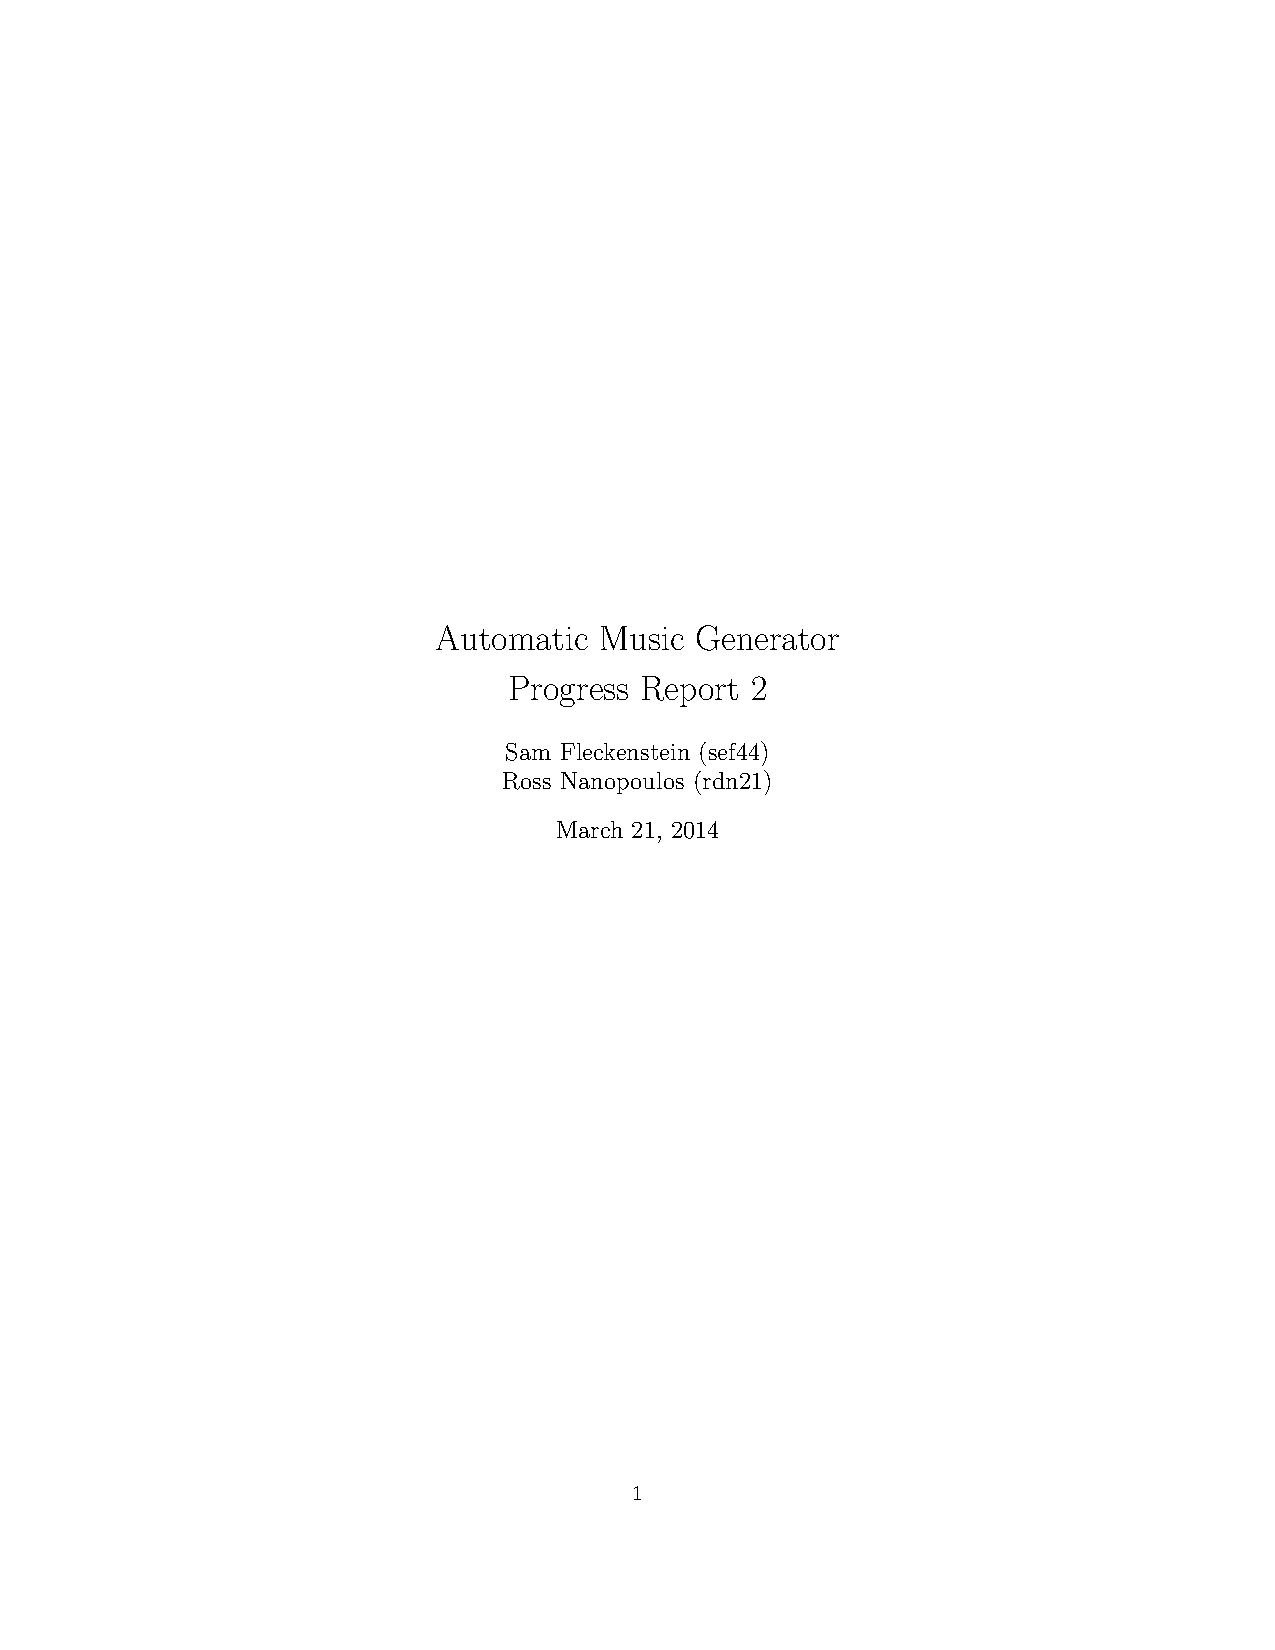
\includepdf[pages=-]{ProgressReport2.pdf}

\end{document}
